\documentclass{article}
\usepackage{amsmath}
\usepackage{graphicx}
\usepackage{fancyhdr}
\usepackage{pgfplots}
\usepackage{bm}
\usepackage{geometry}
\usepackage{pgfplots}
\usepackage{fontspec}


\geometry{left=2.0cm,right=2.0cm,top=2.5cm,bottom=2.5cm}
\pgfplotsset{compat = 1.16}
\setmainfont{Consolas}

\title{Test tex!}
\author{NUAA}
\date{Janurary 2021}

\pagestyle{fancy}
\renewcommand{\headrulewidth}{0pt}
\renewcommand{\headrulewidth}{0pt}

\fancyhf{}
\rhead{
	NUAA XuTao
}
\rfoot{Page \thepage}

\begin{document}
	
\maketitle

\section*{Introduction}

\begin{enumerate}

\item Let's begin with a formula $e^{i\pi}+1=0$

$$e = \lim_{n\to\infty} \left(1+\frac{1}{n}\right)^n=
\lim_{n\to\infty}\frac{n}{\sqrt[n]{n!}}$$

\item we can do another:

$$ e = \sum_{n=0}^{\infty} \frac{1}{n}.$$

\item we can also use continued fractions:

$$ e = 2 + \frac{1}{1+\frac{2}{2+\frac{3}{3+\frac{4}{4+\frac{5}{5+\ddots}}}}} $$
 
\end{enumerate}

\section*{More formulas}

$$\int_a^b{f(x)}dx$$

$$\iiiint f(x,y,z)dxdydz$$

$$\vec{v}=<v_1,v_2,v_3>$$

$$\vec{v}\cdot \vec{w}$$

$$\left[\begin{matrix}
1 & 2 & 3\\
4 & 5 & 6\\	
\end{matrix}\right]
$$

\begin{center}
	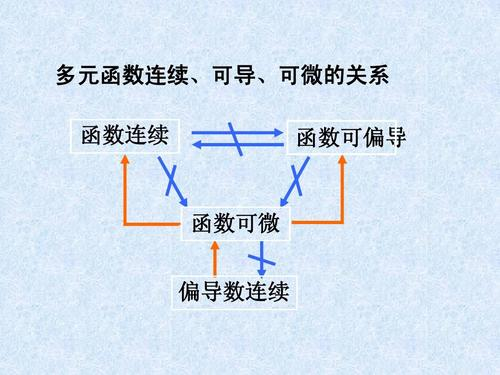
\includegraphics[scale = 0.5]{function.jpg}
\end{center}

\paragraph{1.1}
	\textit{
		\textbf{A} find the sum of $34$ and $126$ using a caculator.
	}
	$$ 34 + 126 = \framebox{$160$} $$
	\textit{
		\textbf{B} Find the sum using long addition.
	}
	\begin{center}
		\begin{tabular}{cccc}
			&   & 1 & 0\\
			&   & 3 & 4\\
		+	& 1 & 2 & 6\\
		\hline
			& 1 & 6 & 0 \\
		\end{tabular}
	\end{center}
\paragraph{1.2}
	\textit{
		Evaluate the following definite integral:
		$$
		\int_{0}^{3} 2x \sqrt{x^2+4} dx
		$$
	}
	$$
		u = x^2 + 4
		\quad %tab
		du = 2x 
	$$
	$$
		\Rightarrow\quad
		\int_{0^2+4}^{3^2+4} \sqrt{u} du 
		= \left. \frac{1}{2} u^{-\frac{1}{2}}
		\right|_{4}^{13}
	$$
	$$
	 \frac{1}{2\sqrt{13}}-
	 \frac{1}{2\sqrt{4}}
	 \approx \framebox{$-0.1113$}
	$$
\paragraph{2.1}
\textit{
	\textbf{A} Find the root of the 
	quadratic equation $y=x^2 +2x -3 $
	using the quadratic formula.
}
$$
	x = \frac{-b\pm\sqrt{b^2-4ac}}{2a}
$$
\section{\textit{Weighted Residual Methods}}
\textbf{Fundamental equations} Consider the problem governed by the differential equation:
$$ \bm{\Gamma u = -\overline{f}}\quad in\;D $$
\textit{The above differential equation is solved by using the boundary conditions given as follows:}
$$
\bm{u=-\overline{u}}\quad on\;S_u
$$
$$
\bm{t\equiv Bu = \overline{t}}\quad on\;S\!\setminus\!S_t
$$
\textit{where the boundary $S$ consists of $S_t$ and $S_u$.\;The boundary conditions given in eqs.$(84)$ and $(85)$ are called rigid and natural boundary conditions,or Dirichlet and Neumann
boundary conditions,respectively.\;In most engineering problems,$\bm{\Gamma}$ and $\bm{B}$ are different operators in the forms of $bm{\Gamma} = \bm{\Delta\cdot\varSigma}$ and $\bm{B}=
\bm{n\cdot\varSigma}$,where $\varsigma$ is another differential operators and $\bm{n}$ is the normal vector on $S_t$.}
$$
\Delta^2 u = -\;\overline{f}\quad in\;D,
$$
\end{document}